\subsection{Calculation of $v_{e}$ and $v_{e}$ vs. Self-Speed Filter}

As the emergency braking system should only react to stationary targets, only the points of those targets should be passed to the next stage, the clustering stage.
Filtering out all points that might be invalid or from moving targets ensures a reliable operation of the clustering process and also effectively reduces processing time as a result of the smaller amount of points.
This filtering operation was implemented using a simplistic approach by assuming that theoretically all points of stationary targets should show a velocity equal to the vehicle's velocity when the radar sensor is moving with the vehicle.
By comparing the points' velocities to the prior obtained self-speed, invalid points or those of dynamic targets can be separated and filtered out.
Due to the working principle of radars and the resulting radar sensor's output format, the dependency between the radial speed and the point's angle to the radar sensor must be taken into account.
\par
The whole block was separated into two sub-stages following after each other.
In the first sub-stage, the angle-independent points' speeds, called $v_{e,p}$, are calculated. 
The following sub-stage executes the filtering operation by comparing the points' $v_{e,p}$ to the vehicle's velocity, supplied by the Kalman filter's output.
The calculation of $v_{e,p}$ followed the same approach that was used in the self-speed estimator.
An angle $\phi_{p}$ was defined between each individual point $p$ of the point cloud and the radar sensor's centerline (see \ref{fig:def_angle_phi}).
This angle is calculated for every point by using the prior presented formula.
The dependency between the point's radial speed $v_{r,p}$ and the calculated angle $\phi_{p}$ is then used to calculate each point's angle-independent speed $v_{e,p}$:
\begin{equation*}
    v_{e,p} = \frac{v_{r,p}}{cos(\phi_{p})}
\end{equation*}
A division by zero never occurs because of the first static filtering stage.
Filtering by $v_{e,p}$ is done by calculating the difference between the estimated vehicle's self-speed and $v_{e,p}$ and comparing it against a threshold.
The comparison of the difference to a threshold is needed as $v_{e,p}$ will rarely be exactly equal to the vehicle's self-speed.
A threshold of \SI{0.5}{\meter\per\second} was found out to be sufficient.
After filtering, the points are passed to the clustering stage.

\begin{figure}[!htbp]
\centering
\begin{subfigure}{0.24\textwidth}
  \centering
  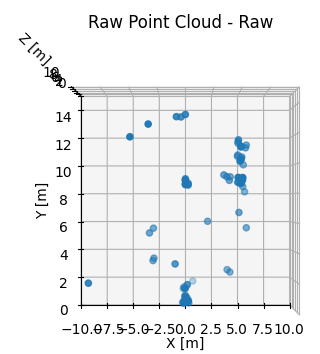
\includegraphics[width=\textwidth]{images/withoutVeFilter.png}
  \caption{Input}
\end{subfigure}
\begin{subfigure}{0.24\textwidth}
  \centering
  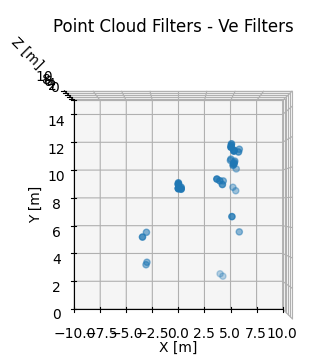
\includegraphics[width=\textwidth]{images/wVeFilter.png}
  \caption{Output}
\end{subfigure}
\caption{Example visualization of the input and output data before and after passing the $v_{e}$ vs. self-speed filtering stage.}
\label{fig:example_ve_filtering_stage}
\end{figure}
\FloatBarrier\noindent